
\chapter{Analysis}\label{chapter:analysis}

The first very important criterion by which implementations are judged is the running time. It plays a crucial role in the decision of using a specific code in real life applications and it is influence by various factors such as the choice of algorithm that is implemented and of the smaller sub procedures that compose the big picture, the programming language, i.e. instruction set in this case, the implementation details that many times make an important difference, the decisions about the trade-off between code complexity and time, the hardware capabilities and so on. The analysis is split into two parts: judging if the expected running time the implementation of each step of the algorithm is met and comparing the total number of cycles with other works. 

\section{Cycle Count per Step}

To check if there is no unexpected bottle neck, one needs to check each of the 7 implementation steps and make sure they do not take more clock cycles than they should. The total cycle count of the algorithm for a random input is 34420. The following diagram shows how these cycles are distributed among the steps:

\vspace{5mm}

\begin{tikzpicture}

\pie[radius=3]{8.1/SNORT $\&$ reordering,
    3.6/multiplication by $X^i$,
    19.6/forward butterfly,
    28.2/large number multiplication,
    9.8/backward butterfly,
    4.6/multiplication by $X^{-i}$ $\&$ $t^{-1}$,
    26.1/SNEEZE $\&$ reordering $\&$ reduction by q}

\end{tikzpicture}

The first two steps are rather fast which is to be expected since their implementations are also relatively short and without too long loops. The forward butterfly (applied to both inputs) takes a big part of the total running time, which is also to be expected since the NTT is on of the main operations in the algorithm. It is interesting to note that the time of the forward NTT is double the time of the backward NTT (applied only to the result) which is again expected since a large part of the implementation of the two is shared and the other parts are similar. The large number multiplication is the most time consuming part, which is again expected since this is the part one tries to reduce. A larger $t$ would reduce this part even further but will increase the other steps. Step 6 turns out to be inexpensive thanks to not computing the full large number multiplication but just a multiplication by one 64-bit chunk. The last part is the surprising bit even if a couple of steps are compressed into one pass through the coefficients. To understand which parts are expensive, the following figure shows the percentage of number of cycles for each sub-step of step 7:

\vspace{5mm}

\begin{tikzpicture}

\pie[radius=2]{33.1/coefficient loading $\&$ extraction $\&$ storing,
    44.1/SNEEZE,
    22.8/modulo reduction}

\end{tikzpicture}

There are 256 numbers that need to be processed, which means running each instruction in the processing pipeline 256 times. Some instructions take 2 cycles instead of 1 as well. Reducing the code by one instruction in this setting translates into a great reduction in the number of cycles. The coefficient extraction is slow since multiple 64-bit chunks are read into WDRs instead of 32-bit registers in order to make the SNEEZE and modulo reduction simpler. The extraction alone takes 8 instructions, mostly because the instruction set is not perfectly fitted for this use case. One of these instruction takes 2 cycles, hence the extraction takes $9 \cdot 256 = 2304$ cycles. From the diagram it does not seem that one part is excessively expensive but rather all of them are moderately expensive. The issue is that there are many coefficients and the each instruction adds many cycles. Through analyzing the code in detail one may be able to reduce the number of instructions by finding another way to implement the same operations. This would make a significant improvement, but keeping in mind that the first part of the algorithm, namely preprocessing, forward NTT and the multiplication are to be executed $k$ times when the second part is executed only once (due to the aggregation in the NTT domain improvement), the issue is to some degree ameliorated.

To continue the analysis, it would be useful to imagine what would happen for other parameter choices: increasing t to 16 would decrease the numbers' widths by a factor of 2 and so the running time of the multiplication by a factor of 4. On the other hand, it would increase both the running time of steps 2, 3, 5 and 6 by a factor of 2. Computing the expected running time for the set of parameters $l=64, t=16$, it seems that the choice $t=8$ is by far better. Decreasing t to 4 would increase the running time of the multiplication by a factor of 4 but decrease the number of cycles for the other mentioned steps by a factor of 2. This makes the number of cycles of multiplication already larger than the number of cycles of the whole algorithm in the current setting. Changing $l$ to a smaller number which is not a power of 2 (since it needs to stay above 54), makes a couple of steps as the coefficient reordering, Kroneker substitution operations and others a lot more complex to implement. The extra complexity translates into more instructions which means more cycles. The difference in the numbers' widths is relatively small, hence this wouldn't be an improvement.

\section{Comparison with other implementations of polynomial multiplication schemes}

To evaluate the quality of the implementation, the overall running time is compared with a couple other implementations of polynomial multiplication schemes. One needs to keep in mind that since these other implementations are tuned for other polynomial rings, they were written with different instruction sets and have been evaluated on different hardware, the comparison is rather rough.

In the setting of Dilithium, keeping in mind that ultimately a matrix vector multiplication will be performed, the time consumption can be split into the preprocessing and forward NTT regarded together, the multiplication, and the backward NTT and postprocessing. Table \ref*{tab:comparison} shows cycle counts split into these there categories for a couple of polynomial multiplications implementations for Dilithium. It should be noted that both the Cortex M3 and M4 processors have more advanced hardware and a larger instruction set but they do not have such a large multiplier (64 bits) as OTBN has. Given that, the proposed implementation ranks pretty well in between the ones for Cortex M3 and Cortex M4.

The last entry in the table is a C implementation on OpenTitan's main processor of the polynomial multiplication as given in the Dilithium scheme. This represents the alternative to a using the big number accelerator of OpenTitan. If one holds an OpenTitan processor and wants to implement Dilithium on it, the benefit of using the implementation given in this work is clearly visible since the running time is almost three times lower and because the OpenTitan's main processor would meanwhile be free to process other things. 


\begin{table}[htpb]
    \caption[]{}\label{tab:comparison}
    \centering
    \begin{tabular}{p{0.4\linewidth} | p{0.15\linewidth} | p{0.07\linewidth} | p{0.15\linewidth} | p{0.07\linewidth}}
      \toprule
         Work & Preprocess $\&$ NTT & Mult & Postprocess $\&$ INTT & Total \\
      \midrule
         Faster Kyber and Dilithium on the Cortex-M4~\parencite{10.1007/978-3-031-09234-3_42} & 8093 & 1955 & 8415 & 18463  \\
         \hline
         \textbf{This Work} & \textbf{10763} & \textbf{9714} & \textbf{13943} & \textbf{34420} \\
         \hline
         Compact Dilithium Implementations on Cortex-M3 and Cortex-M4 ~\parencite{cryptoeprint:2020/1278} (M3 version) & 19347 & 4899 & 21006 & 45252 \\
         \hline 
         Dilithium baseline OpenTitan & 40002 & 7455 & 46649 & 94106 \\

      \bottomrule
    \end{tabular}
  \end{table}

  Aside from comparison with other implementations, it is important to note what would be the benefits of having a larger multiplier. Increasing the multiplier by a factor of two would reduce the multiplication cost by a factor of 4 which would permit to decrease t to 4 which would increase the multiplication time by a factor of 4 getting back to the current running time. The benefit would be that the number of cycles of the steps 2, 3, 5 and 6 would decrease by a factor of 2, potentially by a large amount. Increasing the multiplier to a full 256-bit size would permit to also decrease the multiplication time by a factor of 4 when keeping $t=4$. From these considerations one understands that the Kroneker+ algorithm largely benefits from having a large multiplier as RSA and ECC dedicated processors have, even if direct application of the NTT for numbers modulo $q = 2^{23} - 2^{13} + 1$ does not benefit from that.